\documentclass[journal,12pt,twocolumn]{IEEEtran}
\usepackage{amsmath,amssymb,amsfonts}
\usepackage{cancel}
\usepackage{graphicx}
\usepackage{float}
\title{Assignment 1}
\author{\Large{Name : Harshit Pant}\\\Large{Roll Number : CS21BTECH11021}}
\date{}
\begin{document}
\maketitle
\setlength{\parindent}{0cm}
\textbf{Q.6(c) [ICSE 2018] :}
Prove that,\\[.1in]
$(1 +\cot\theta -\csc\theta)(1 + \tan\theta +\sec\theta)=2$\\[.1in]
\textbf{Solution : }
\begin{align}
\text{L.H.S.}&=(1+ \cot\theta -\csc\theta)(1+\tan\theta+\sec\theta)\\[.1in]
\begin{split}
&=1+\cot\theta-\csc\theta+\tan\theta+\tan\theta\cot\theta\\[.1in]
&\qquad-\tan\theta\csc\theta+\sec\theta+\sec\theta\cot\theta\\[.1in]
&\qquad-\sec\theta\csc\theta\\[.1in]
\end{split}\\[.1in]
\begin{split}
&=\displaystyle{2+\cot\theta-\csc\theta+\tan\theta}\\[.1in]
&\qquad
\displaystyle{-\frac{\cancel{\sin\theta}}{\cos\theta}\frac{1}{\cancel{\sin\theta}}+\sec\theta+\frac{1}{\cancel{\cos\theta}}\frac{\cancel{\cos\theta}}{\sin\theta}}\\[.1in]
&\qquad
-\sec\theta\csc\theta
\end{split}\\[.1in]
\begin{split}
&=2+\cot\theta-\cancel{\csc\theta}+\tan\theta-\cancel{\sec\theta}\\[.1in]
&\qquad+\cancel{\sec\theta}+\cancel{\csc\theta}-\sec\theta\times\csc\theta\\[.1in]
\end{split}\\[.1in]
&=2+\dfrac{\cos\theta}{\sin\theta}+\dfrac{\sin\theta}{\cos\theta}-\sec\theta\times\csc\theta\\[.1in]
&=\displaystyle{2+\dfrac{{\cos}^2\theta+{\sin}^2\theta}{\sin\theta\times\cos\theta}-\sec\theta\times\csc\theta}\\[.1in]
\begin{split}
&=\displaystyle{2+\frac{1}{\sin\theta\times\cos\theta}-\sec\theta\times\csc\theta}\\[.1in]
&\hspace{1.2in}
(\because{\cos}^2\theta+{\sin}^2\theta=1)\\[.1in]
\end{split}\\[.1in]
&=\displaystyle{2+\cancel{\csc\theta\times\sec\theta}-\cancel{\sec\theta\times\csc\theta}}\\[.1in]
&=2
\end{align}
\\\textbf{\Large{Output}}
\begin{figure}[H]
\begin{center}
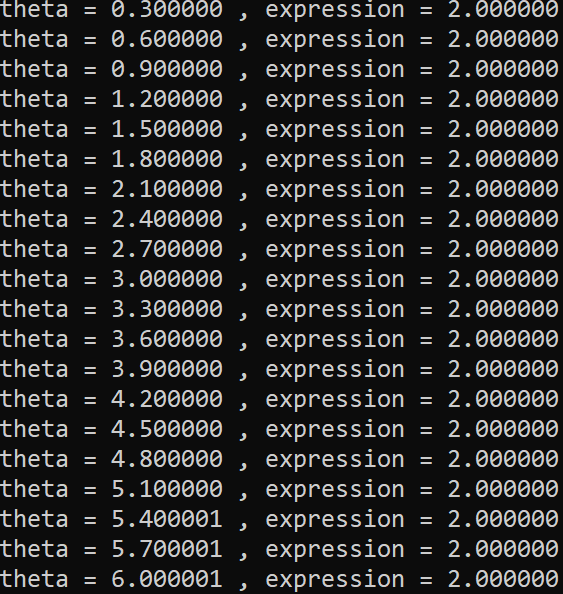
\includegraphics[width=2.75in]{fig.png}
\end{center}
\end{figure}

\end{document}